\section{Motivation and research question}

Security analysts use logs to connect scattered operations that may belong to the same attack. Human operators and AI agents may follow different operational patterns, making execution mode a potentially useful context for interpreting behavioral evidence. We study whether predicting execution mode from logs helps activity correlation recover missed links while controlling spurious links.

Behavioral association is an established computational task: HOLMES correlates suspicious information flows in host-audit traces to produce campaign evidence; OSTINATO compares behavior and TTPs across hosts; POIROT and ActMiner align CTI-derived attack graphs with provenance graphs; HERCULE, ATLAS, and FALCON reconstruct multi-stage attack stories from correlated logs \cite{holmes,ostinato,poirot,actminer,hercule,atlas,falcon}. These methods use command or event sequences, TTPs, entity relations, and causal structure as evidence. Their evaluation targets differ, but each demonstrates a concrete role for behavioral association in investigation. Practitioner frameworks likewise track activity clusters before assigning named actors \cite{unit42}.

Execution mode is now part of the observable threat narrative. Anthropic's 2025 report describes human operators coordinating Claude Code agents and MCP tools across a multi-stage campaign; MITRE records the activity as Campaign C0062 \cite{anthropic,mitrec0062}. These developments motivate execution mode as a new dimension of behavioral analysis: helping analysts interpret operational differences, connect scattered evidence, and enrich threat characterization as human, scripted, and Agent execution coexist. AIT/AECID provides adjacent log-based Human/LLM classification for IT troubleshooting \cite{ait}. We explore the next question: how can predicted execution-mode information contribute to activity association?

\section{Data and protocol}

We use the pinned CC BY 4.0 release of Cyber Task Horizons (revision \texttt{178c0da1800f9\allowbreak c07311e1b8d\allowbreak 6c61dd8104e7b\allowbreak 4e7b4ae}) \cite{cth}. It contains task-based CTF evaluations and expert terminal recordings. We select InterCode-CTF, CyBench, and NYU CTF Bench, the three suites with overlapping human and Agent task records. The resulting corpus has 177 non-empty traces in 40 benchmark-qualified task groups: 57 expert terminal records and 120 Agent tool-call records. InterCode-CTF contributes 27 groups (40 human, 81 Agent), CyBench 6 (8 human, 18 Agent), and NYU CTF Bench 7 (9 human, 21 Agent).

\begin{table}[t]
\centering
\caption{Trace sources in the evaluated intersection.}
\label{tab:data}
\small
\rowcolors{2}{PaleGray}{white}
\begin{tabularx}{0.84\linewidth}{>{\raggedright\arraybackslash}Xrrr}
\toprule
\rowcolor{InkBlue}\textcolor{white}{Benchmark} & \textcolor{white}{Task groups} & \textcolor{white}{Human} & \textcolor{white}{Agent} \\
\midrule
InterCode-CTF & 27 & 40 & 81 \\
CyBench & 6 & 8 & 18 \\
NYU CTF Bench & 7 & 9 & 21 \\
\rowcolor{PaleBlue}\textbf{Total} & \textbf{40} & \textbf{57} & \textbf{120} \\
\bottomrule
\end{tabularx}
\end{table}

Human records are terminal-input transcripts; Agent records are structured bash tool calls. For both, we extract allowlisted command names and coarse action categories. Prompts, task descriptions, outputs, model names, timestamps, and paths are excluded; 300 Python calls are omitted from primary features. The release instructs human experts not to use AI, but remote collection cannot independently verify this. The labels therefore describe released trace sources, not independently adjudicated decision-maker identity.

The primary protocol uses three benchmark-stratified outer folds grouped by benchmark/task, with seed \texttt{20261030}. Every query is ranked against all other held-out traces from the same benchmark and fold, with no mode filtering; the mean gallery contains 29.325 candidates. The evaluation label records whether two traces solve the same benchmark-qualified challenge. It is not a shared intrusion, activity, campaign, or actor label. Five additional seeds estimate split sensitivity. Task groups are the unit of metric aggregation and bootstrap resampling. We report task-macro \Hit, mean reciprocal rank (MRR), Recall@5, and nDCG@5. Intervals use 5,000 paired benchmark-stratified task-cluster bootstrap draws conditional on fitted folds.

The behavior ranker combines command cosine, ordered action-bigram cosine, ProcGrep BPE/Jensen--Shannon similarity, and command-length similarity. A task-supervised ranker learns from same-task versus different-task pairs. The mode-aware ranker adds execution-mode scores generated out of fold within each training partition. Pair labels depend only on task identity; test labels and source metadata are excluded from inference. ProcGrep is a pinned third-party adaptation, not a method introduced by this project.

\section{Results}

\subsection{Initial mixed-gallery retrieval protocol}

The mixed gallery gives a random-ranking \Hit{} of 0.189. Command cosine reaches 0.600; ProcGrep reaches 0.594; the task-supervised behavior ranker reaches 0.571. Mode-aware ranking is highest on the fixed primary split at 0.607, a +0.036 paired change over the task-supervised ranker (95\% CI [+0.006, +0.069]). Against command cosine, the change is +0.008 (95\% CI [−0.046, +0.059]). Across the five alternate splits, the mode-aware minus task-supervised change averages −0.007 (95\% CI [−0.026, +0.012]). The positive primary-split estimate therefore does not persist across the split-sensitivity check.

\begin{table}[t]
\centering
\caption{Mixed-gallery task retrieval on the primary split. Higher is better.}
\label{tab:retrieval}
\small
\rowcolors{2}{PaleGray}{white}
\begin{tabularx}{\linewidth}{>{\raggedright\arraybackslash}Xrrrr}
\toprule
\rowcolor{InkBlue}\textcolor{white}{Method} & \textcolor{white}{\Hit} & \textcolor{white}{MRR} & \textcolor{white}{Recall@5} & \textcolor{white}{nDCG@5} \\
\midrule
Command TF--IDF cosine & 0.600 & 0.695 & 0.648 & 0.618 \\
Action bigram cosine & 0.565 & 0.657 & 0.591 & 0.567 \\
ProcGrep BPE/JSD & 0.594 & 0.676 & 0.551 & 0.544 \\
Length only & 0.514 & 0.636 & 0.543 & 0.514 \\
Task-supervised behavior & 0.571 & 0.669 & 0.600 & 0.576 \\
\rowcolor{PaleBlue}\textbf{Mode-aware behavior} & \textbf{0.607} & \textbf{0.693} & \textbf{0.619} & \textbf{0.604} \\
Mode only & 0.281 & 0.483 & 0.433 & 0.366 \\
\bottomrule
\end{tabularx}
\end{table}

\begin{figure}[t]
\centering
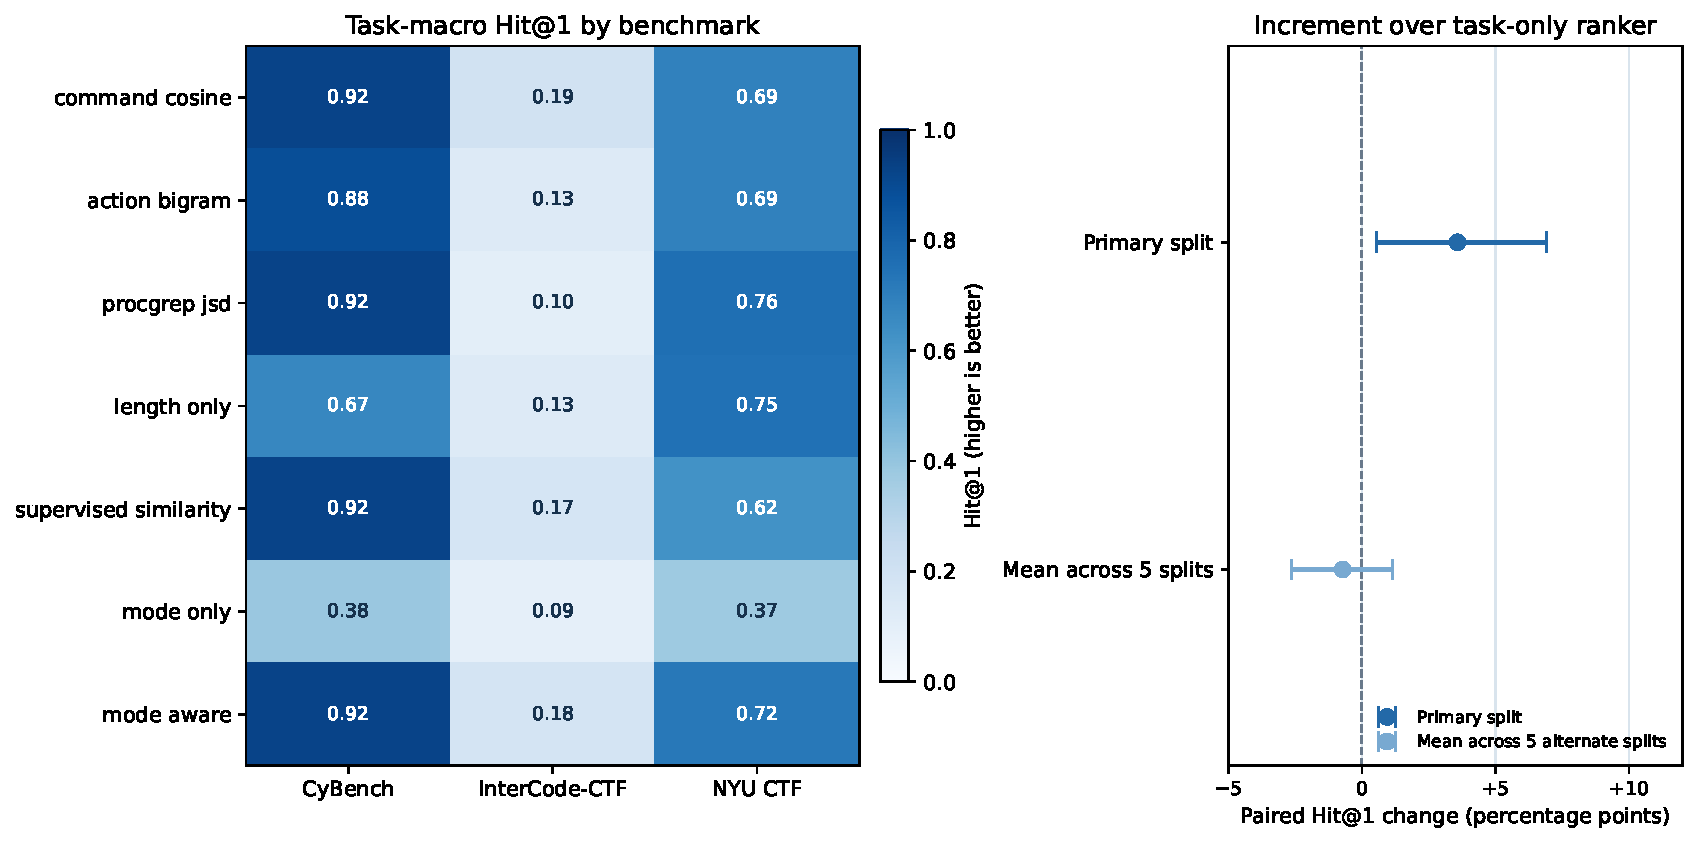
\includegraphics[width=\linewidth]{mixed_gallery_retrieval.pdf}
\caption{Benchmark-level task retrieval and paired mode-score changes. The right panel shows the primary estimate and the average across five alternate task splits; the dashed line marks no change.}
\label{fig:retrieval}
\end{figure}

At a 0.5 threshold on Platt-calibrated held-out scores, the mode classifier's pooled confusion matrix is $[[43,14],[8,112]]$ for Human/Agent rows, corresponding to record-level balanced accuracy 0.844. Fold scores are 0.912, 0.883, and 0.738. Platt calibration is fit on training-task out-of-fold predictions and reduces test Brier score from 0.110 to 0.089. These measurements show that the two released record types are separable in this corpus. Because label and capture interface coincide, they do not establish recognition of an unknown operator.

\begin{figure}[t]
\centering
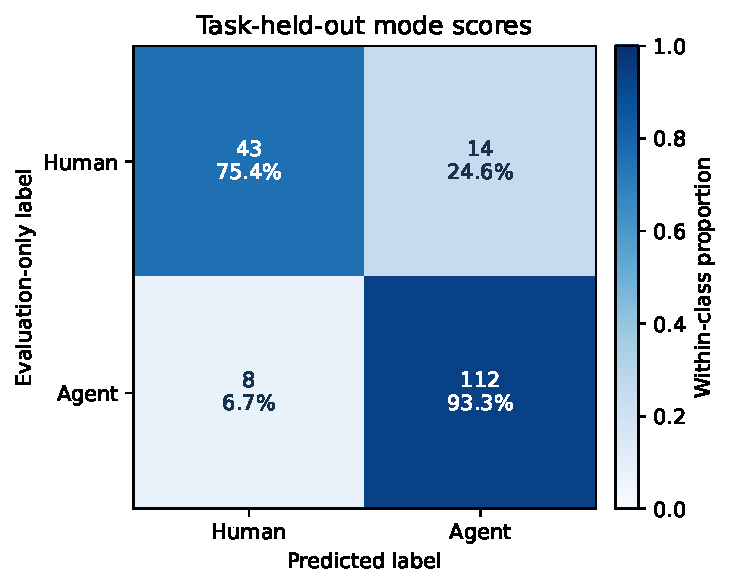
\includegraphics[width=0.63\linewidth]{mixed_gallery_confusion.pdf}
\caption{Task-held-out Human/Agent trace-label confusion matrix. Cells show counts and within-class proportions.}
\label{fig:confusion}
\end{figure}

\subsection{Association errors at a training-only threshold}

Retrieval metrics do not show the errors made when the system decides whether to connect a pair. We therefore evaluate pairwise decisions under a nested protocol: each outer training fold supplies three inner task-held-out folds for threshold selection; the outer test tasks remain untouched. Each method receives its own threshold, selected to maximize task-macro balanced accuracy on inner out-of-fold pairs. A test pair is linked when its score meets that threshold. We compare command cosine, the task-supervised behavior ranker, its mode-aware extension, and a command-length control. The target is same-task matching within the released CTF benchmarks, not real attack-activity matching.

The mode-aware ranker reaches task-macro balanced accuracy 0.669 (95\% task-cluster CI [0.611, 0.722]), compared with 0.612 [0.568, 0.657] for the behavior-only ranker. The paired increase is 5.7 percentage points [3.4, 8.1]. Against command cosine, however, the increase is 0.6 points [−4.1, 4.8], leaving no clear gain over this simpler baseline.

The pair-type breakdown shows where the mode score changes decisions. Relative to behavior-only ranking, it lowers the false-split rate for same-task H--Agent pairs from 0.317 to 0.191 (−12.6 points, 95\% CI [−17.7, −7.6]) while raising the false-merge rate for different-task H--Agent pairs from 0.387 to 0.472 (+8.4 points, [3.4, 13.2]). Execution-mode context therefore reduces one cross-mode matching error while increasing another; the result supports conditional use of this signal, not a universal correction.

\begin{table}[t]
\centering
\caption{Task-held-out pairwise association errors. Each method's decision threshold is selected on inner training-task out-of-fold pairs. Entries are task-macro rates with 95\% task-cluster bootstrap intervals. Relevance labels denote the same CTF challenge.}
\label{tab:association-errors}
\small
\rowcolors{2}{PaleGray}{white}
\begin{tabularx}{\linewidth}{>{\raggedright\arraybackslash}Xrrr}
\toprule
\rowcolor{InkBlue}\textcolor{white}{Method} & \textcolor{white}{False split} & \textcolor{white}{False merge} & \textcolor{white}{Balanced accuracy} \\
\midrule
Command cosine & 0.377 [0.288, 0.470] & 0.296 [0.198, 0.399] & 0.664 [0.597, 0.731] \\
Task-supervised behavior & 0.275 [0.185, 0.371] & 0.501 [0.433, 0.569] & 0.612 [0.568, 0.657] \\
\rowcolor{PaleBlue}\textbf{Mode-aware behavior} & \textbf{0.238 [0.148, 0.343]} & \textbf{0.423 [0.363, 0.491]} & \textbf{0.669 [0.611, 0.722]} \\
Length-only control & 0.195 [0.122, 0.277] & 0.600 [0.506, 0.689] & 0.602 [0.531, 0.677] \\
\bottomrule
\end{tabularx}
\end{table}

\begin{figure}[t]
\centering
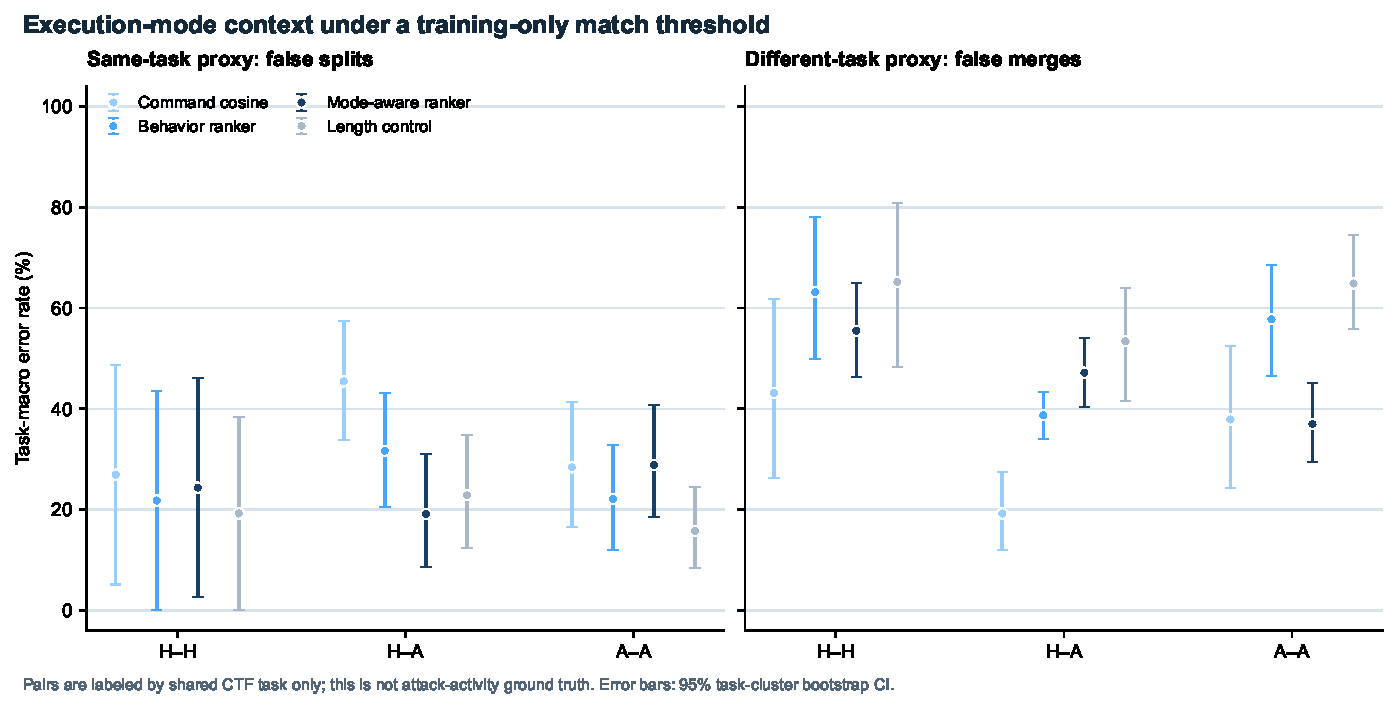
\includegraphics[width=\linewidth]{association_error_rates.pdf}
\caption{False-split and false-merge rates stratified by pair mode. H--A denotes a pair of records labeled Human and Agent in the dataset. The same-task H--H estimate uses 17 task groups; all other strata use 40. Error bars are 95\% task-cluster bootstrap intervals.}
\label{fig:association-errors}
\end{figure}

\subsection{Feature signal and fixed-operating-point association}

We test whether execution-mode labels can be separated from three observable input groups: trace size and coarse action mix, command vocabulary, and fixed sequence statistics. F0–F2 are single-group baselines; F3 combines command vocabulary with sequence statistics. This is a feature ablation for the broader question of whether execution mode can inform behavior-based activity association; it does not define separate dimensions of the research question. The primary ablation is F3 versus F1, which isolates the added value of sequence statistics given command vocabulary. On task-held-out traces, command TF--IDF reaches balanced accuracy (BA) 0.849 with logistic regression and 0.866 with ExtraTrees. Fixed sequence statistics alone reach 0.648 and 0.642. Adding these statistics changes BA by $-2.0$ points for logistic regression (95\% task-cluster CI [$-8.3$, $+3.3$]) and $+1.4$ points for ExtraTrees ([$+0.3$, $+2.5$]); their contribution is classifier-dependent.

\begin{table}[t]
\centering
\caption{Task-held-out execution-mode source-label classification. Values are task-macro BA with 95\% task-cluster intervals.}
\label{tab:feature-ablation}
\small
\rowcolors{2}{PaleGray}{white}
\begin{tabularx}{\linewidth}{>{\raggedright\arraybackslash}Xccc>{\centering\arraybackslash}p{1.55cm}>{\centering\arraybackslash}p{1.55cm}}
\toprule
\rowcolor{InkBlue}\textcolor{white}{Feature set} & \textcolor{white}{Count + action mix} & \textcolor{white}{Command TF--IDF} & \textcolor{white}{Sequence statistics} & \textcolor{white}{Logistic BA} & \textcolor{white}{ExtraTrees BA} \\
\midrule
F0: Coarse baseline & $\bullet$ & -- & -- & 0.643 & 0.635 \\
F1: Command vocabulary & -- & $\bullet$ & -- & 0.849 & 0.866 \\
F2: Sequence structure & -- & -- & $\bullet$ & 0.648 & 0.642 \\
\rowcolor{PaleBlue}\textbf{F3: F1 + structure} & -- & $\bullet$ & $\bullet$ & \textbf{0.828} & \textbf{0.880} \\
\bottomrule
\end{tabularx}
\smallskip
\footnotesize $\bullet$ included; -- excluded. BA is task-macro balanced accuracy (higher is better). The primary ablation, F3 $-$ F1, is $-2.0$ percentage points for Logistic Regression (95\% CI [$-8.3$, $+3.3$]) and $+1.4$ points for ExtraTrees ([$+0.3$, $+2.5$]).
\end{table}

On the matched cohort with at least four commands (99 traces, 25 tasks), full command sequences outperform their first-four-command prefixes by 8.8 points for TF--IDF (95\% CI [+2.0, +15.7]); shuffling command order yields a +3.1-point change whose interval crosses zero. These results locate most measured separability in command content and observation amount, not a stable order signature.

\begin{figure}[t]
\centering
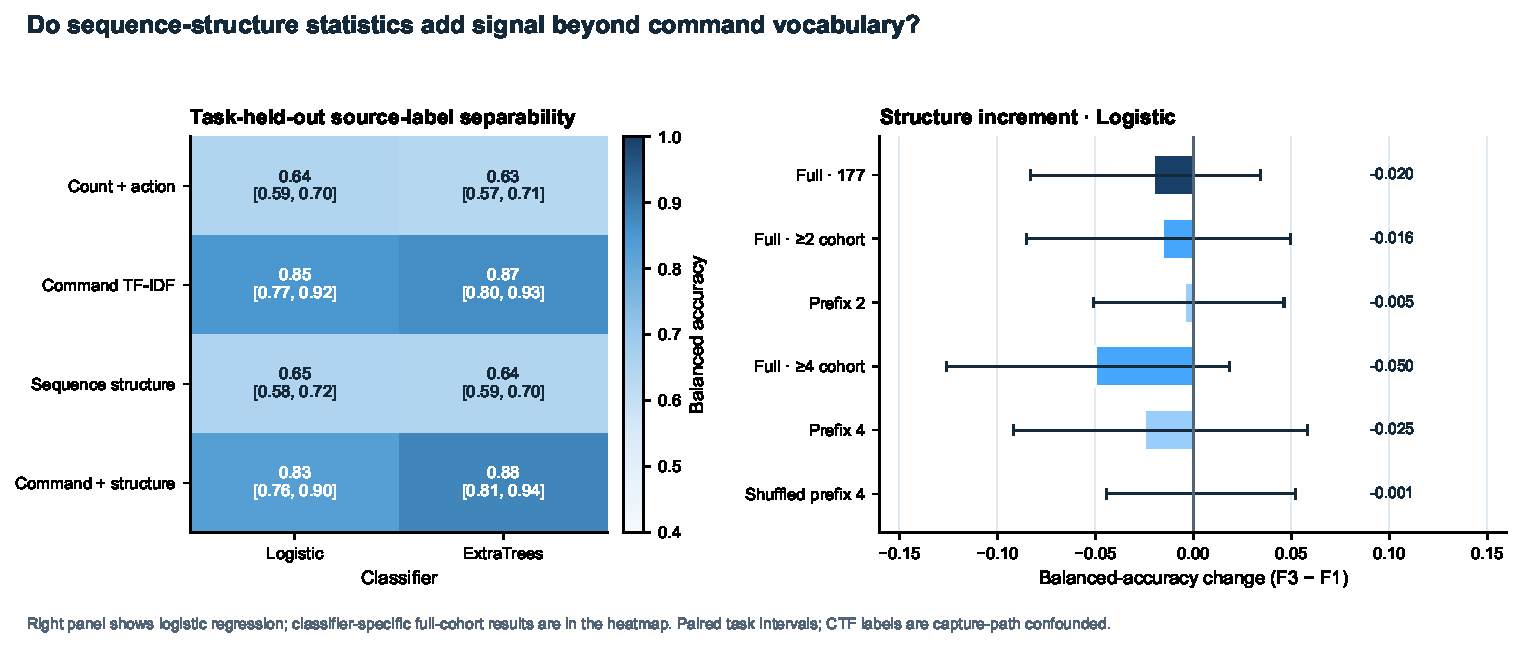
\includegraphics[width=\linewidth]{feature_ablation_v1.pdf}
\caption{Source-label separability and paired feature increments. The right panel shows the logistic-regression increment across matched cohorts; the left panel reports both classifiers. Labels remain confounded with capture interface.}
\label{fig:feature-ablation}
\end{figure}

\begin{figure}[t]
\centering
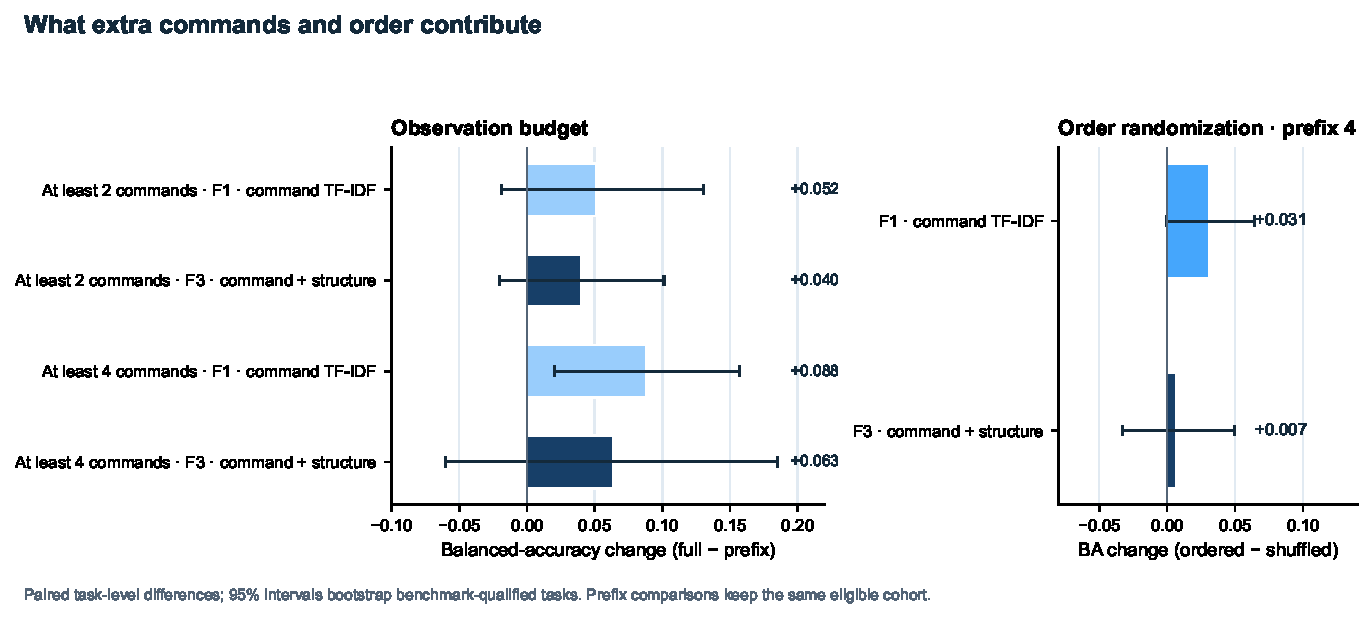
\includegraphics[width=\linewidth]{feature_budget_order_v1.pdf}
\caption{Matched-cohort changes from observing full traces instead of prefixes and from preserving versus shuffling command order.}
\label{fig:feature-budget-order}
\end{figure}

For association, thresholds are selected within each outer training fold to keep task-macro false merges at or below 20\%, then minimize false splits. At this operating point, mode-aware ranking attains Hit@1 0.607 versus 0.571 for the behavior ranker (paired change +3.6 points, 95\% CI [+0.6, +6.8]). Same-task Human--Agent false splits fall by 12.7 points ([$-19.0$, $-6.5$]), while different-task Human--Agent false merges rise by 11.9 points ([$+7.9$, $+16.3$]). The realized test false-merge rates are 24.5\% for mode-aware and 23.3\% for behavior ranking, since the 20\% ceiling is imposed on training data. Command cosine remains competitive (Hit@1 0.600; false merges 10.1\%).

\begin{table}[t]
\centering
\caption{Association results at a 20\% training false-merge target. Entries are task-macro test estimates with 95\% task-cluster intervals.}
\label{tab:operating-point}
\small
\rowcolors{2}{PaleGray}{white}
\begin{tabularx}{\linewidth}{>{\raggedright\arraybackslash}Xrrr}
\toprule
\rowcolor{InkBlue}\textcolor{white}{Ranker} & \textcolor{white}{False split} & \textcolor{white}{False merge} & \textcolor{white}{Hit@1} \\
\midrule
Command cosine & 0.585 [0.471, 0.696] & 0.101 [0.075, 0.126] & 0.600 [0.500, 0.688] \\
Behavior & 0.457 [0.357, 0.563] & 0.233 [0.162, 0.307] & 0.571 [0.485, 0.653] \\
Structure-aware & 0.483 [0.375, 0.593] & 0.218 [0.140, 0.301] & 0.584 [0.482, 0.670] \\
\rowcolor{PaleBlue}\textbf{Mode-aware} & \textbf{0.416 [0.308, 0.528]} & \textbf{0.245 [0.169, 0.326]} & \textbf{0.607 [0.507, 0.689]} \\
Length control & 0.586 [0.535, 0.637] & 0.240 [0.182, 0.298] & 0.514 [0.432, 0.603] \\
\bottomrule
\end{tabularx}
\end{table}

\begin{figure}[t]
\centering
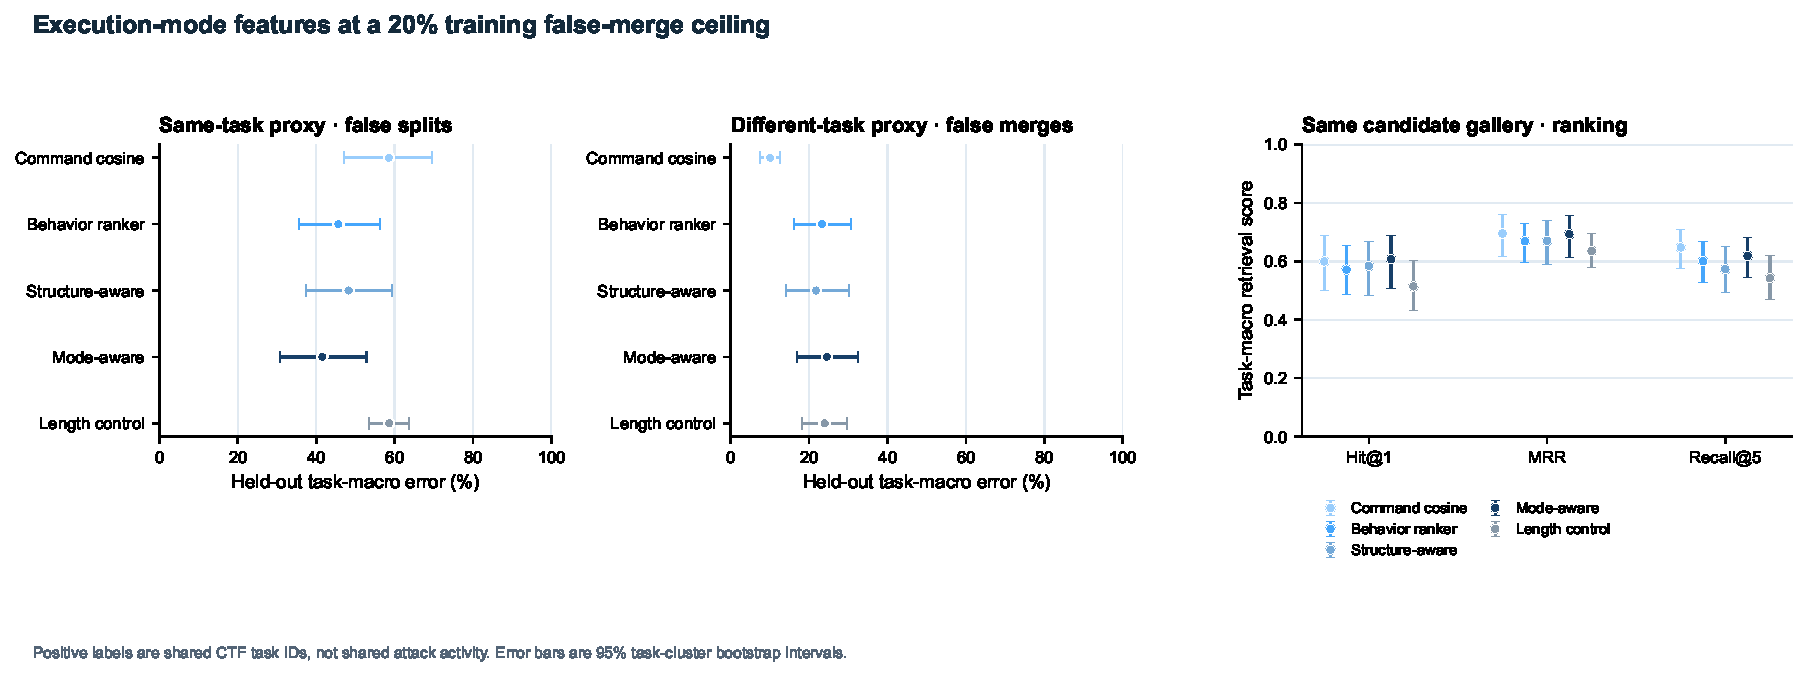
\includegraphics[width=\linewidth]{association_operating_points_v1.pdf}
\caption{Held-out challenge-matching errors and retrieval at the shared training-side 20\% false-merge target. Candidate galleries are identical across methods.}
\label{fig:operating-points}
\end{figure}

% Generated by scripts/plot_association_cases.py from audited JSON.
\subsection{Audited examples of changed decisions}

In the held-out CyBench challenge \texttt{back\_to\_the\_past}, a Human trace with 48 extracted commands and an Agent trace with 47 commands share the task label but have command-cosine similarity 0.215. The behavior ranker rejects the pair ($0.5088 < 0.5131$); the mode-aware ranker accepts it ($0.5482 \geq 0.5127$). The mode detector's raw Agent scores are 0.3683 and 0.7221, respectively. This pair illustrates how predicted mode information can change a borderline matching decision.

The same representation also introduces a cross-challenge link: a Human \texttt{back\_to\_the\_past} trace and an Agent \texttt{glacier-exchange} trace change from rejection ($0.4738 < 0.5131$) to acceptance ($0.5161 \geq 0.5127$). Figure~\ref{fig:association-cases} locates both the value and the design challenge: execution-mode context can recover cross-mode matches, while distinguishing the underlying task remains essential to controlling spurious links. Case selection and full trace identifiers are documented in the appendix.

\begin{figure}[t]
\centering
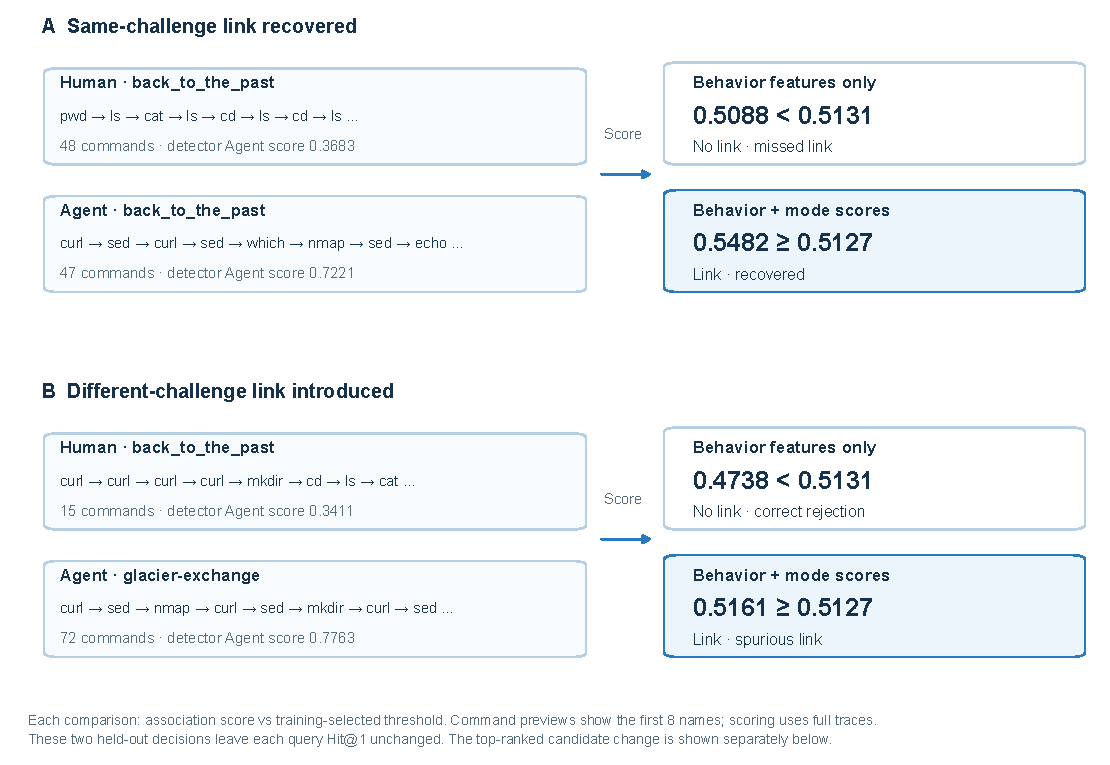
\includegraphics[width=\linewidth]{association_cases_v1.pdf}
\caption{Audited Human--Agent pairs from held-out CTF tasks. Each numeric comparison shows an association score against its training-selected threshold. The common 20\% training false-merge target permits method-specific thresholds. Only command-name previews are displayed; scoring uses complete normalized trajectories. Source labels are shown for interpretation, while the ranker uses predicted mode scores. These examples explain a recovered same-challenge link and a new cross-challenge error.}
\label{fig:association-cases}
\end{figure}


\section{Conclusion}

Security investigations already use sequences, TTPs, and causal relations to associate activity evidence. These experiments show that execution-mode scores can shift this association profile: in CTF same-challenge retrieval, mode-aware ranking recovers more same-task Human--Agent pairs and also introduces more cross-task Human--Agent links. Command vocabulary supplies most of the measured classification signal; sequence statistics add no classifier-independent gain. The results support evaluating execution mode as an explicit association context. The next decisive evaluation requires human, scripted, and Agent executions under one sensor pipeline with independently labeled activities.
